% ======================================================================
% slides_theory.tex — 30-minute 1:1 talk: THEORY ONLY
% Two-period model of formality and finance: results and implications.
% Self-contained (no external inputs); pdfLaTeX.
% Zero identification/estimation content by design.
% ======================================================================
\documentclass[11pt,aspectratio=169]{beamer}
\usetheme{Madrid}
\usecolortheme{dolphin}
\setbeamertemplate{navigation symbols}{}
\setbeamertemplate{footline}[frame number]
\usepackage{amsmath,amssymb,bm}
\usepackage{booktabs}
\usepackage{tikz}
\usetikzlibrary{positioning}
 
% ---- notation (matches the paper) ------------------------------------
\providecommand{\infml}{i}
\providecommand{\fml}{f}
\providecommand{\curv}{\gamma}
\providecommand{\prodx}{x}
\providecommand{\prodxhat}{\hat{x}}
\providecommand{\spread}[1]{\phi_{#1}}
\providecommand{\collat}[1]{b_{#1}}
\providecommand{\Fin}[1]{\Phi_{#1}}
\providecommand{\Rint}{R^{0}}
\providecommand{\Rext}[1]{R_{#1}}
\providecommand{\fc}[1]{c_{#1}}
\providecommand{\ec}[1]{c^{e}_{#1}}
\providecommand{\swc}[1]{c_{#1}}
\providecommand{\death}[1]{\lambda_{#1}}
\providecommand{\taxy}{\tau_{y}}
\providecommand{\taxl}{\tau_{\ell}}
\providecommand{\Om}[1]{\Omega_{#1}}
\providecommand{\netw}{n}
\providecommand{\thF}[1]{\hat{x}^{\mathrm{F}}_{#1}}
\providecommand{\thX}[1]{\hat{x}^{\mathrm{X}}_{#1}}
\providecommand{\thE}[1]{\hat{x}^{\mathrm{E}}_{#1}}
\providecommand{\Uv}[1]{U_{#1}}
\providecommand{\Kop}[1]{\mathcal{K}_{#1}}
\providecommand{\Xth}[1]{\mathcal{X}_{#1}}
\providecommand{\E}{\mathbb{E}}
\providecommand{\Prob}{\mathbb{P}}
\providecommand{\ind}[1]{\mathbf{1}\{#1\}}
\providecommand{\diff}{\mathrm{d}}
 
\title[Formality and finance: theory]{ Model of firms transitions and financial conditions}
\subtitle{Closed-form version}
\author{Costas' meeting}
\date{September 11th, 2026}
 
\begin{document}
 
\begin{frame}
\titlepage
\end{frame}
 
% ----------------------------------------------------------------------
\begin{frame}{Refresher: The question, the evidence, and the theory}

\textbf{Question}: Is firm informality sensitive to the credit conditions?

\vspace{8mm}
\textbf{Evidence}: Yes, the shift-share IV shows that credit 1) $\uparrow$ formal entry, 2) $\uparrow$ informal-formal transitions, and 3) $\downarrow$ formal-informal transitions. 
 
\vspace{8mm}
\textbf{Mechanism}: Formality trades fiscal cost (taxes) w/financial benefit (cheaper external funds, more pledgeable collateral).
 
\vspace{8mm}
\textbf{Theory implications:}
\begin{itemize}
    \item Four regimes of desired capital and internal funds that define the constraint of a firm;
    \item Threshold rules for every entry, exit, and switching margin that depend on financial primitives for constraint firms (cost $\spread{s}$ and collateral $\collat{s}$).
\end{itemize}

\end{frame}

% ----------------------------------------------------------------------
\begin{frame}{Previous discussion: Where this paper stands on the field}

\begin{enumerate}
    \item Fazzari–Hubbard–Petersen: Sort firms by retention and get cash-flow sensitivity.
    \vspace{3mm}
    \item Devereux–Schiantarelli: Sorting on size, age, and sector. Larger firms are more sensitive.
    \vspace{3mm}
    \item Bond–Meghir (BM): Hierarchy of finance w/three endogenous regimes, R1: $D>0$, $N=0$; R2, constrained: $D=0$, $N=0$; R3: $D=0$, $N>0$.
    \vspace{3mm}
    \item Exogenous credit supply shock: Khwaja–Mian, Chodorow-Reich, Greenstone et al.
\end{enumerate}

\vspace{5mm}

\textbf{This paper}: Market level exogenous shifter with four endogenous financial regimes.

\end{frame}
 
% ----------------------------------------------------------------------
\begin{frame}{Environment: two periods, two sectors, two frictions}
\begin{columns}[T]
\column{0.52\textwidth}
\textbf{Technology and heterogeneity}
\begin{itemize}
    \item $y=\theta k^{\alpha}\ell^{\nu}$, $\alpha+\nu<1$
    \item $\ln\theta_{1}=\ln v+\varepsilon_{1}+u_{1}$,\;
    $\ln\theta_{2}=\rho\ln\theta_{1}+(1-\rho)\ln v+\varepsilon_{2}+u_{2}$
\end{itemize}
\vspace{3mm}
\textbf{Fiscal side}
\begin{itemize}
  \item formal: revenue tax $\taxy$, payroll tax $\taxl$
  \item informal: evades both; lower fixed cost
    $\fc{\infml}<\fc{\fml}$
\end{itemize}
\column{0.44\textwidth}
\textbf{Financial side (sector-specific)}
\begin{itemize}
  \item Funds $a$ cost $\Fin{s}(a)=\spread{s}a$,\;
    $\spread{\infml}>\spread{\fml}$
  \item collateral: $a\leq\collat{s}k'$,\;
    $\collat{\infml}<\collat{\fml}$
\end{itemize}
\vspace{3mm}
\textbf{Transitions}
\begin{itemize}
  \item entry fees $\ec{s}$, switch fees
    $\swc{\infml\fml},\swc{\fml\infml}$
  \item exogenous death $\death{s}$; depreciation $\delta$
\end{itemize}
\end{columns}

\vspace{5mm}
\textbf{Timing:} Decisions depend on expected productivity only, before shocks are observed.

\vspace{5mm}
\textbf{Implication}: Entry, exit, and formality decisions are a cutoff in productivity $\prodxhat=\E\big[\prodx_{2}\mid\varepsilon_{1},v\big]$.
\end{frame}
 
% ----------------------------------------------------------------------
\begin{frame}{Investment and financing: a four-region policy}
User costs $\;\Rint=1-\beta(1-\delta)$ (internal),
$\;\Rext{s}=\Rint+\spread{s}$ (external); targets
$\bar k_{s}>\tilde k_{s}$ solve $\mathrm{MPK}=\Rint,\Rext{s}$.

\begin{center}
\renewcommand{\arraystretch}{1.25}\small
\begin{tabular}{lllll}
\toprule
 & funds $\netw$ vs.\ targets & capital $k^{*}_{s}$ &
 borrowing $a^{*}_{s}$ & cash sens.\ \\
\midrule
R1: unconstrained (BM's R1) & $\netw\geq\bar k_{s}$ & $\bar k_{s}(\prodxhat)$
 & 0 & 0 \\
R2: kink (self-financed) (BM's R2) & $\tilde k_{s}\leq\netw<\bar k_{s}$ &
 $\netw$ & 0 & 1 \\
R3: interior borrowing (BM's R3) & $(1-\collat{s})\tilde k_{s}\leq\netw
 <\tilde k_{s}$ & $\tilde k_{s}(\prodxhat)$ & $\tilde k_{s}-\netw$
 & 0 \\
R4: collateral-capped (BM's R2) & $\netw<(1-\collat{s})\tilde k_{s}$ &
 $\dfrac{\netw}{1-\collat{s}}$ & $\collat{s}k^{*}_{s}$ &
 $\dfrac{1}{1-\collat{s}}$ \\
\bottomrule
\end{tabular}
\end{center}

\medskip
\structure{Take away:} Financial cost moves intensive margin of
R3 borrowers; collateral moves the most constrained firms (R4: young, low-wealth); cash-flow sensitivity only where constraints bind.

\medskip
\begin{itemize}
    \item Bond-Meghir regime 2 is split in two: price constrained and quantity constrained.  
\end{itemize}

\end{frame}
 
% ----------------------------------------------------------------------
\begin{frame}{Operating values respond through borrowing}
Value of operating: $\Uv{s}(\prodxhat,\netw)=\netw
+G_{s}(\prodxhat,\netw)-\beta(1-\death{s})\fc{s}$, with $G_{s}$ in
closed form. The marginal value of a peso inside the firm,
\begin{equation*}
  q_{s}=1+\frac{\partial G_{s}}{\partial\netw}:\qquad
  \underbrace{1}_{\text{R1}}\;\;<\;\;
  \underbrace{(1,\,1+\spread{s}]}_{\text{R2}}\;\;
  \underbrace{=1+\spread{s}}_{\text{R3}}\;\;<\;\;
  \underbrace{1+\spread{s}
  +\tfrac{\mathrm{MPK}-\Rext{s}}{1-\collat{s}}}_{\text{R4}}
\end{equation*}

By the envelope theorem, for each sector $s$:
\begin{equation*}
  \frac{\partial\Uv{s}}{\partial\spread{s}}=-\,a^{*}_{s}\;\leq 0,
  \qquad\qquad
  \frac{\partial\Uv{s}}{\partial\collat{s}}=\mu_{s}k^{*}_{s}\;\geq 0,
  \qquad\qquad
  \frac{\partial\Uv{s}}{\partial\spread{s'}}
  =\frac{\partial\Uv{s}}{\partial\collat{s'}}=0 .
\end{equation*}
 
\medskip
\structure{Consequence:} every comparative static is one of these two objects divided by a slope, financial conditions
matter only where firms are constrained.
\end{frame}
 
% ----------------------------------------------------------------------
\begin{frame}{The formality margin: single crossing}
For origin $o$ (entrant, $\infml$-incumbent, $\fml$-incumbent) with
funds $\netw_{o}$ and on the borrowing region, the formal-vs-informal
comparison is \emph{affine} in $\prodxhat^{1/(1-\curv)}$:
\begin{equation*}
  \Delta_{o}(\prodxhat)=A\,\prodxhat^{\frac{1}{1-\curv}}
  -B\,\netw_{o}-C_{o},\qquad
  B=\spread{\infml}-\spread{\fml}>0 .
\end{equation*}
\textbf{Assumption (finance-driven formality):}
$\big(\Rext{\fml}/\Rext{\infml}\big)^{\curv}<T_{\lambda}
\iff A>0$: the financing advantage outweighs the fiscal cost
(adjusted by survival, $T_{\lambda}=T\cdot
\tfrac{1-\death{\fml}}{1-\death{\infml}}$).
 
\begin{equation*}
  \Rightarrow\quad
  \boxed{\;\thF{o}(\netw_{o})
  =\Big[\frac{B\,\netw_{o}+C_{o}}{A}\Big]^{1-\curv},\qquad
  \frac{\partial\thF{o}}{\partial\netw_{o}}>0\;}
\end{equation*}
 
\structure{Sorting result:} formal firms are those with \emph{high
growth needs relative to internal wealth}.
\begin{itemize}
    \item Conditional on expected productivity, etc., \emph{richer} firms are \emph{less} likely to formalize, self-finance substitutes for the financial advantage of formality.
\end{itemize}

\end{frame}
 
% ----------------------------------------------------------------------
\begin{frame}{Ordered thresholds}
Each origin's
policy is a partition of the $\prodxhat$ line:
$ \thX{\infml} < \thE{\infml} < \thX{\fml} < \thF{\fml} < \thF{e} < \thF{\infml} $

\begin{center}
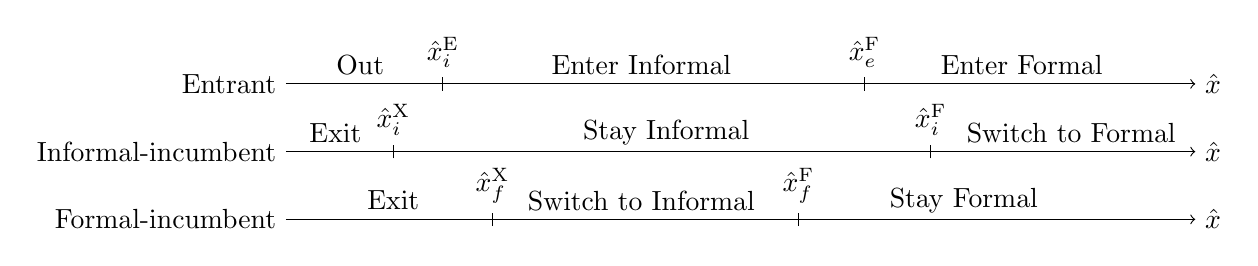
\begin{tikzpicture}[xscale=1.05, yscale=0.86, every node/.style={font=\normalsize}]
  % entrant line
  \draw[->] (0,2) -- (11,2) node[right] {$\prodxhat$};
  \node[left] at (0,2) {Entrant};
  \foreach \x/\lab in {1.9/{$\thE{\infml}$}, 7.0/{$\thF{e}$}}
    \draw (\x,1.9) -- (\x,2.1) node[above] {\lab};
  \node at (0.9,2.28) {Out};
  \node at (4.3,2.28) {Enter Informal};
  \node at (8.9,2.28) {Enter Formal};
  % informal incumbent
  \draw[->] (0,1) -- (11,1) node[right] {$\prodxhat$};
  \node[left] at (0,1) {Informal-incumbent};
  \foreach \x/\lab in {1.3/{$\thX{\infml}$}, 7.8/{$\thF{\infml}$}}
    \draw (\x,0.9) -- (\x,1.1) node[above] {\lab};
  \node at (0.6,1.28) {Exit};
  \node at (4.6,1.28) {Stay Informal};
  \node at (9.5,1.28) {Switch to Formal};
  % formal incumbent
  \draw[->] (0,0) -- (11,0) node[right] {$\prodxhat$};
  \node[left] at (0,0) {Formal-incumbent};
  \foreach \x/\lab in {2.5/{$\thX{\fml}$}, 6.2/{$\thF{\fml}$}}
    \draw (\x,-0.1) -- (\x,0.1) node[above] {\lab};
  \node at (1.3,0.28) {Exit};
  \node at (4.3,0.28) {Switch to Informal};
  \node at (8.2,0.28) {Stay Formal};
\end{tikzpicture}
\end{center}

\end{frame}
 
% ----------------------------------------------------------------------
\begin{frame}{Exit and entry threshold, four regimes}
Every margin solves $G_{\infml}(\prodxhat,\tilde\netw)=m$
(continuation vs.\ consuming the outside value; the informal option is
the relevant alternative at low $\prodxhat$):
\begin{equation*}
  \Xth{s}(\tilde\netw;m)=
  \begin{cases}
    (m/A^{0}_{s})^{1-\curv} & \text{Region 1, independent of finance}\\[2pt]
    \dfrac{m+\Rint\tilde\netw}{M_{s}\tilde\netw^{\curv}}
      & \text{Region 2}\\[6pt]
    \Big[\dfrac{m-\spread{s}\tilde\netw}{A_{s}}\Big]^{1-\curv}
      & \text{Region 3}\\[6pt]
    (1-\collat{s})^{\curv}\,
    \dfrac{m+\tilde\netw\frac{\Rint+\spread{s}\collat{s}}
    {1-\collat{s}}}{M_{s}\tilde\netw^{\curv}} & \text{Region 4}
  \end{cases}
\end{equation*}

\end{frame}
 
% ----------------------------------------------------------------------
\begin{frame}{Comparative statics of all thresholds: signs and exclusions}
\begin{center}
\renewcommand{\arraystretch}{1.55}\small
\begin{tabular}{lcccc}
\toprule
 & $\spread{\fml}\uparrow$ & $\spread{\infml}\uparrow$ &
 $\collat{\fml}\uparrow$ & $\collat{\infml}\uparrow$ \\
\midrule
formality margins $\thF{e},\thF{\infml},\thF{\fml}$ &
$\dfrac{(1-\curv)a^{*}_{\fml}}{D_{o}}>0$ &
$-\dfrac{(1-\curv)a^{*}_{\infml}}{D_{o}}<0$ & $\leq0$ & $\geq0$ \\
informal entry/exit $\thE{\infml},\thX{\infml}$ & $0$ &
$\dfrac{a^{*}_{\infml}}{\Psi'_{\infml}}>0$ & $0$ & $\leq0$ \\
formal exit $\thX{\fml}$ & $0$ &
$\dfrac{a^{*}_{\infml}}{\Psi'_{\infml}}>0$ & $0$ & $\leq0$ \\
\bottomrule
\end{tabular}
\end{center}
\medskip
\begin{itemize}
  \item Every effect is an envelope object: $\pm a^{*}$ or $\pm\mu k^{*}$ with a slope, \emph{effects scale with borrowing at the margin}.
  \item With infinite horizon the crossed financial conditions become second-order (re-switching options), the sign pattern survives.
\end{itemize}
\end{frame}
 
% ----------------------------------------------------------------------
\begin{frame}{From thresholds to transition probabilities}
Conditional on $(v,\netw)$: $\ln(\theta_{1})\sim N(\ln v,
\sigma_{\varepsilon}^{2})$ and decisions are cutoffs in $\theta_{1}$,
so every transition is a probit-type object:
\begin{equation*}
  \Prob(\infml\to\fml\mid v,\netw)=1-\Phi(z),\qquad
  z=\frac{\ln\bar\theta(v,\netw)-\ln v}{\sigma_{\varepsilon}},
\end{equation*}
and every response to financial conditions has the form
\begin{equation*}
  \frac{\partial p}{\partial(\text{financial parameter})}
  =\pm\,\underbrace{\phi(z)}_{\substack{\text{density of}\\
  \text{marginal firms}}}\times
  \underbrace{\frac{1-\nu}{\rho\,\sigma_{\varepsilon}}}_{\text{units}}
  \times
  \underbrace{\frac{a^{*}\ \text{or}\ \mu k^{*}}{\text{slope}}}
  _{\text{envelope term}} .
\end{equation*}
\structure{Aggregation:} responses are incidence-weighted integrals: largest where the firm distribution is thick near thresholds
(young, small, low-wealth firms); unconstrained firms contribute
zero.
\end{frame}
 
% ----------------------------------------------------------------------

\begin{frame}[noframenumbering]{}

\centering
\Huge
E S T I M A T I O N

\end{frame}
 
% ----------------------------------------------------------------------

\begin{frame}{Results of model estimated parameters}
\begin{center}
\renewcommand{\arraystretch}{1.12}
\begin{tabular}{llrrll}
\toprule
Param. & Assigned moment & Data & Model & Status & Reason \\
\midrule
$\mu_{ko}$ & mean entrant $k$ (inf.) & 1.966 & 1.967 & hit
 \;(s.e.\ 0.211) & n.a. \\
$\sigma_{ko}$ & p90 entrant $k$ (inf.) & 3.871 & 2.416 & ceiling & fat-tail K0 \\
$\phi_{0f}$ & borrowing incid.\ (for.) & 0.177 & 0.176 & hit
 \;(s.e.\ 0.773) & n.a. \\
$\phi_{0i}$ & borrowing incid.\ (inf.) & 0.098 & 0.098 &
 hit \;(s.e.\ 0.240) & n.a. \\
$c_i$ & exit 5y (inf.) & 0.351 & 0.350 & hit
 \;(s.e.\ 0.001) & n.a. \\
$c_f$ & exit 5y (for.) & 0.279 & 0.258 & bound & partial match \\
$c_{if}$ & switch 5y $\infml{\to}\fml$ & 0.059 & 0.041 &
 floor & Cost $\to$ 0 \\
$c_{fi}$ & switch 5y $\fml{\to}\infml$ & 0.365 & 0.245 &
 floor & Size-composition \\
$c^e_f$ & formal entry share & 0.063 & 0.046 & floor & Size-composition  \\
$c^e_i$ & entrant rel.\ size (inf.) & $-0.142$ & $-0.095$ & floor & partial match  \\
\bottomrule
\end{tabular}
\end{center}
\smallskip
Four exactly estimated and six corner solutions.
\end{frame}
 
% ----------------------------------------------------------------------

\begin{frame}{Verification evidence}

\begin{itemize}
  \item \textbf{Multistart}: 8 random draws over the
    admissible box yield consistent estimations.
  \item \textbf{Jacobian}: Dominance verified at $\widehat\theta$, 3 out of 4: informal borrowing-incidence, $\phi_{0i}$, fails.
  \item \textbf{Threshold ordering.} The assumed exit / own-sector /
    formal ordering holds \emph{exactly} at $\widehat\theta$.
\end{itemize}

\begin{center}
    \includegraphics[scale=0.49]{slides_material/fig_jacobian_heatmap.pdf}
    \includegraphics[scale=0.48]{slides_material/fig_policy_partition.pdf}
\end{center}

\end{frame}
 
% ----------------------------------------------------------------------
\begin{frame}{Validation results}

\textbf{LOO-SSIV on model-simulated markets}:

\begin{center}
    \renewcommand{\arraystretch}{1.2}
    \begin{tabular}{lcccccc}
        \toprule
         & \# inf. firms & entry & inf.\ exit & $\infml{\to}\fml$ &
         $\fml{\to}\infml$ & avg.\ VA \\
        \midrule
        Data $\hat\beta$ & $0.173$ & $0.192$ & $0.205$ & $0.195$ &
         $0.113$ & $-0.073$ \\
        Model $\hat\beta$ & $0.023$ & $0.016$ & $-0.092$ & $-0.256$ & $0.119$ &
         $0.053$ \\
        \bottomrule
    \end{tabular}
\end{center}

\medskip
\begin{itemize}
  \item \textbf{\# firms and entry}: right-signed, strongly attenuated.
  \item \textbf{Switching pair} ($\infml{\to}\fml$, $\fml{\to}\infml$): Opposite directions by construction. 
  \begin{itemize}
      \item Taste shock on formality: i-f moment exact, incidence and size-entrant improved, but deteriorates informal exit. 
  \end{itemize}
  \item \textbf{Informal exit}: Cheaper informal credit reduces informal exit ($-0.09$), but in data rises ($+0.21$).
\end{itemize}

\end{frame}
 
% ----------------------------------------------------------------------
\begin{frame}{Counterfactuals}

\begin{center}
    \renewcommand{\arraystretch}{1.2}
    \begin{tabular}{lrr}
        \toprule
        Counterfactual & $\Delta$ For-share (pp) & $\Delta\ln$ agg.\ VA (\%) \\
        \midrule
        $\varphi_i \to \varphi_f$ & $-0.44$ & $-1.14$ \\
        $b_i \to b_f$ & $-0.16$ & $+0.42$ \\
        $\varphi_{0i} \to \varphi_{0f}$ & $+3.70$ & $-0.76$ \\
        All financing & $+3.76$ & $-0.48$ \\
        $\tau_i \to \tau_f$ & $+0.92$ & $+0.67$ \\
        \bottomrule
    \end{tabular}
\end{center}

\medskip
\begin{itemize}
  \item Formalization most sensitive financial parameter: Fixed borrowing cost, $\varphi_{0i}$.
  \item Small VA effects in the model, as in the LOO-SSIV.
\end{itemize}
\end{frame}
 
% ----------------------------------------------------------------------

\begin{frame}{General questions}

\begin{itemize}
    \item Readiness for the market (w/sound reduced-form but improvement space in estimation)?
    \vspace{8mm}
    \item Alternatives to going to the market?
\end{itemize}

\end{frame}
 
% ----------------------------------------------------------------------
 
\end{document}